\section{Гамильтоновы циклы и цепи в графе. Теоремы Дирака и Оре. Выяснить, существует ли в 
указанном графе Гамильтонов цикл.}

\begin{definition}
    Граф называется \textit{гамильтоновым}, если существует простой
    цикл, проходящий по всем вершинам графа.
\end{definition}

\begin{definition}
    Граф называется \textit{полугамильтоновым}, если существует простая
    цепь, проходящая через все вершины графа.
\end{definition}

Покажем, что понятия эйлерова и гамильтонова графа не связаны между
собой, то есть у графов могут встретиться всевозможные комбинации этих
понятий.

\begin{figure}[h]
    \centering
    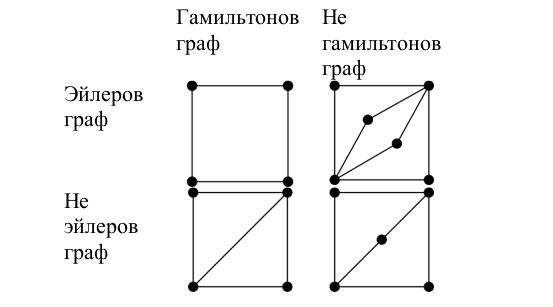
\includegraphics[scale=0.4]{23.png}
\end{figure}

Критерия гамильтонова графа нет. Но есть достаточные условия
гамильтоновости графа. Теоремы Дирака и Оре связывают понятие
гамильтоновости со степенями $\delta(v)$ вершин графа.

\begin{theorem}
    \textbf{Дирака}. Если $n \geq 3$ и $\delta(v) \geq n/2$ для любой вершины $v$
    неориентированного графа $G$, то $G$ -- гамильтонов граф.
\end{theorem}

\begin{theorem}
    \textbf{Оре}. Если $n \geq 3$ и $\delta(u) + \delta(v) \geq n$ для любых двух различных
    несмежных вершин $u, v$ неориентированного графа $G$, то $G$ -- гамильтонов граф.
\end{theorem}